% Options for packages loaded elsewhere
\PassOptionsToPackage{unicode}{hyperref}
\PassOptionsToPackage{hyphens}{url}
%
\documentclass[
]{book}
\usepackage{amsmath,amssymb}
\usepackage{lmodern}
\usepackage{ifxetex,ifluatex}
\ifnum 0\ifxetex 1\fi\ifluatex 1\fi=0 % if pdftex
  \usepackage[T1]{fontenc}
  \usepackage[utf8]{inputenc}
  \usepackage{textcomp} % provide euro and other symbols
\else % if luatex or xetex
  \usepackage{unicode-math}
  \defaultfontfeatures{Scale=MatchLowercase}
  \defaultfontfeatures[\rmfamily]{Ligatures=TeX,Scale=1}
\fi
% Use upquote if available, for straight quotes in verbatim environments
\IfFileExists{upquote.sty}{\usepackage{upquote}}{}
\IfFileExists{microtype.sty}{% use microtype if available
  \usepackage[]{microtype}
  \UseMicrotypeSet[protrusion]{basicmath} % disable protrusion for tt fonts
}{}
\makeatletter
\@ifundefined{KOMAClassName}{% if non-KOMA class
  \IfFileExists{parskip.sty}{%
    \usepackage{parskip}
  }{% else
    \setlength{\parindent}{0pt}
    \setlength{\parskip}{6pt plus 2pt minus 1pt}}
}{% if KOMA class
  \KOMAoptions{parskip=half}}
\makeatother
\usepackage{xcolor}
\IfFileExists{xurl.sty}{\usepackage{xurl}}{} % add URL line breaks if available
\IfFileExists{bookmark.sty}{\usepackage{bookmark}}{\usepackage{hyperref}}
\hypersetup{
  pdftitle={Data Science for Biologists - 5023Y},
  pdfauthor={Philip Leftwich},
  hidelinks,
  pdfcreator={LaTeX via pandoc}}
\urlstyle{same} % disable monospaced font for URLs
\usepackage{color}
\usepackage{fancyvrb}
\newcommand{\VerbBar}{|}
\newcommand{\VERB}{\Verb[commandchars=\\\{\}]}
\DefineVerbatimEnvironment{Highlighting}{Verbatim}{commandchars=\\\{\}}
% Add ',fontsize=\small' for more characters per line
\usepackage{framed}
\definecolor{shadecolor}{RGB}{248,248,248}
\newenvironment{Shaded}{\begin{snugshade}}{\end{snugshade}}
\newcommand{\AlertTok}[1]{\textcolor[rgb]{0.94,0.16,0.16}{#1}}
\newcommand{\AnnotationTok}[1]{\textcolor[rgb]{0.56,0.35,0.01}{\textbf{\textit{#1}}}}
\newcommand{\AttributeTok}[1]{\textcolor[rgb]{0.77,0.63,0.00}{#1}}
\newcommand{\BaseNTok}[1]{\textcolor[rgb]{0.00,0.00,0.81}{#1}}
\newcommand{\BuiltInTok}[1]{#1}
\newcommand{\CharTok}[1]{\textcolor[rgb]{0.31,0.60,0.02}{#1}}
\newcommand{\CommentTok}[1]{\textcolor[rgb]{0.56,0.35,0.01}{\textit{#1}}}
\newcommand{\CommentVarTok}[1]{\textcolor[rgb]{0.56,0.35,0.01}{\textbf{\textit{#1}}}}
\newcommand{\ConstantTok}[1]{\textcolor[rgb]{0.00,0.00,0.00}{#1}}
\newcommand{\ControlFlowTok}[1]{\textcolor[rgb]{0.13,0.29,0.53}{\textbf{#1}}}
\newcommand{\DataTypeTok}[1]{\textcolor[rgb]{0.13,0.29,0.53}{#1}}
\newcommand{\DecValTok}[1]{\textcolor[rgb]{0.00,0.00,0.81}{#1}}
\newcommand{\DocumentationTok}[1]{\textcolor[rgb]{0.56,0.35,0.01}{\textbf{\textit{#1}}}}
\newcommand{\ErrorTok}[1]{\textcolor[rgb]{0.64,0.00,0.00}{\textbf{#1}}}
\newcommand{\ExtensionTok}[1]{#1}
\newcommand{\FloatTok}[1]{\textcolor[rgb]{0.00,0.00,0.81}{#1}}
\newcommand{\FunctionTok}[1]{\textcolor[rgb]{0.00,0.00,0.00}{#1}}
\newcommand{\ImportTok}[1]{#1}
\newcommand{\InformationTok}[1]{\textcolor[rgb]{0.56,0.35,0.01}{\textbf{\textit{#1}}}}
\newcommand{\KeywordTok}[1]{\textcolor[rgb]{0.13,0.29,0.53}{\textbf{#1}}}
\newcommand{\NormalTok}[1]{#1}
\newcommand{\OperatorTok}[1]{\textcolor[rgb]{0.81,0.36,0.00}{\textbf{#1}}}
\newcommand{\OtherTok}[1]{\textcolor[rgb]{0.56,0.35,0.01}{#1}}
\newcommand{\PreprocessorTok}[1]{\textcolor[rgb]{0.56,0.35,0.01}{\textit{#1}}}
\newcommand{\RegionMarkerTok}[1]{#1}
\newcommand{\SpecialCharTok}[1]{\textcolor[rgb]{0.00,0.00,0.00}{#1}}
\newcommand{\SpecialStringTok}[1]{\textcolor[rgb]{0.31,0.60,0.02}{#1}}
\newcommand{\StringTok}[1]{\textcolor[rgb]{0.31,0.60,0.02}{#1}}
\newcommand{\VariableTok}[1]{\textcolor[rgb]{0.00,0.00,0.00}{#1}}
\newcommand{\VerbatimStringTok}[1]{\textcolor[rgb]{0.31,0.60,0.02}{#1}}
\newcommand{\WarningTok}[1]{\textcolor[rgb]{0.56,0.35,0.01}{\textbf{\textit{#1}}}}
\usepackage{longtable,booktabs,array}
\usepackage{calc} % for calculating minipage widths
% Correct order of tables after \paragraph or \subparagraph
\usepackage{etoolbox}
\makeatletter
\patchcmd\longtable{\par}{\if@noskipsec\mbox{}\fi\par}{}{}
\makeatother
% Allow footnotes in longtable head/foot
\IfFileExists{footnotehyper.sty}{\usepackage{footnotehyper}}{\usepackage{footnote}}
\makesavenoteenv{longtable}
\usepackage{graphicx}
\makeatletter
\def\maxwidth{\ifdim\Gin@nat@width>\linewidth\linewidth\else\Gin@nat@width\fi}
\def\maxheight{\ifdim\Gin@nat@height>\textheight\textheight\else\Gin@nat@height\fi}
\makeatother
% Scale images if necessary, so that they will not overflow the page
% margins by default, and it is still possible to overwrite the defaults
% using explicit options in \includegraphics[width, height, ...]{}
\setkeys{Gin}{width=\maxwidth,height=\maxheight,keepaspectratio}
% Set default figure placement to htbp
\makeatletter
\def\fps@figure{htbp}
\makeatother
\setlength{\emergencystretch}{3em} % prevent overfull lines
\providecommand{\tightlist}{%
  \setlength{\itemsep}{0pt}\setlength{\parskip}{0pt}}
\setcounter{secnumdepth}{5}
\usepackage{booktabs}
\usepackage{amsthm}
\makeatletter

\newenvironment{kframe}{%
\medskip{}
\setlength{\fboxsep}{.8em}
 \def\at@end@of@kframe{}%
 \ifinner\ifhmode%
  \def\at@end@of@kframe{\end{minipage}}%
  \begin{minipage}{\columnwidth}%
 \fi\fi%
 \def\FrameCommand##1{\hskip\@totalleftmargin \hskip-\fboxsep
 \colorbox{shadecolor}{##1}\hskip-\fboxsep
     % There is no \\@totalrightmargin, so:
     \hskip-\linewidth \hskip-\@totalleftmargin \hskip\columnwidth}%
 \MakeFramed {\advance\hsize-\width
   \@totalleftmargin\z@ \linewidth\hsize
   \@setminipage}}%
 {\par\unskip\endMakeFramed%
 \at@end@of@kframe}
\makeatother

\makeatletter
\@ifundefined{Shaded}{
}{\renewenvironment{Shaded}{\begin{kframe}}{\end{kframe}}}
\makeatother

\newenvironment{block}[1]
  {
  \begin{itemize}
  \renewcommand{\labelitemi}{
    \raisebox{-.7\height}[0pt][0pt]{
      {\setkeys{Gin}{width=3em,keepaspectratio}\includegraphics{images/#1}}
    }
  }
  \setlength{\fboxsep}{1em}
  \begin{kframe}
  \item
  }
  {
  \end{kframe}
  \end{itemize}
  }
\newenvironment{rmdnote}
  {\begin{block}{note}}
  {\end{block}}
\newenvironment{rmdtip}
  {\begin{block}{tip}}
  {\end{block}}
\newenvironment{rmdwarning}
  {\begin{block}{warning}}
  {\end{block}}
  
\def\thm@space@setup{%
  \thm@preskip=8pt plus 2pt minus 4pt
  \thm@postskip=\thm@preskip
}
\makeatother
\ifluatex
  \usepackage{selnolig}  % disable illegal ligatures
\fi
\usepackage[]{natbib}
\bibliographystyle{apalike}

\title{Data Science for Biologists - 5023Y}
\author{Philip Leftwich}
\date{2021-09-27}

\begin{document}
\maketitle

{
\setcounter{tocdepth}{1}
\tableofcontents
}
\hypertarget{introduction}{%
\chapter{Introduction}\label{introduction}}

\hypertarget{approach-and-style}{%
\section{Approach and style}\label{approach-and-style}}

This book is designed to accompany the module BIO-5023Y for those new to R looking for best practices and tips. So it must be both accessible and succinct. The approach here is to provide just enough text explanation that someone very new to R can apply the code and follow what the code is doing. It is not a comprehensive textbook.

A few other points:

This is a code reference book accompanied by relatively brief examples - not a thorough textbook on R or data science

This is intended to be a living document - optimal R packages for a given task change often and we welcome discussion about which to emphasize in this handbook

Top tips for the course:

\textbf{DON'T} worry if you don't understand everything

\textbf{DO} ask lots of questions!

\hypertarget{teaching}{%
\section{Teaching}\label{teaching}}

We have:

\begin{itemize}
\tightlist
\item
  one lecture per week
\item
  one workshop per week
\end{itemize}

These are both timetabled in-person sessions, and you should check \href{https://timetabler.uea.ac.uk/Timetable}{Timetabler} for up to-date information on scheduling. However, all lessons can be accessed remotely through Collaborate, and \textbf{everything} you need to complete workshops will be available on this site.

If you feel unwell, or cannot attend a session in-person because you need to self-isolate then don't worry you can access everything, and follow along in real time, or work at your own pace.

Questions/issues/errors can all be posted on our \href{https://web.yammer.com/main/groups/eyJfdHlwZSI6Ikdyb3VwIiwiaWQiOiI3OTAyMTk1NzEyMCJ9/all}{Yammer} page.

\hypertarget{workshops}{%
\subsection{Workshops}\label{workshops}}

The workshops are the best way to learn, they teach you the practical skills you need to become an R wizard

\begin{figure}
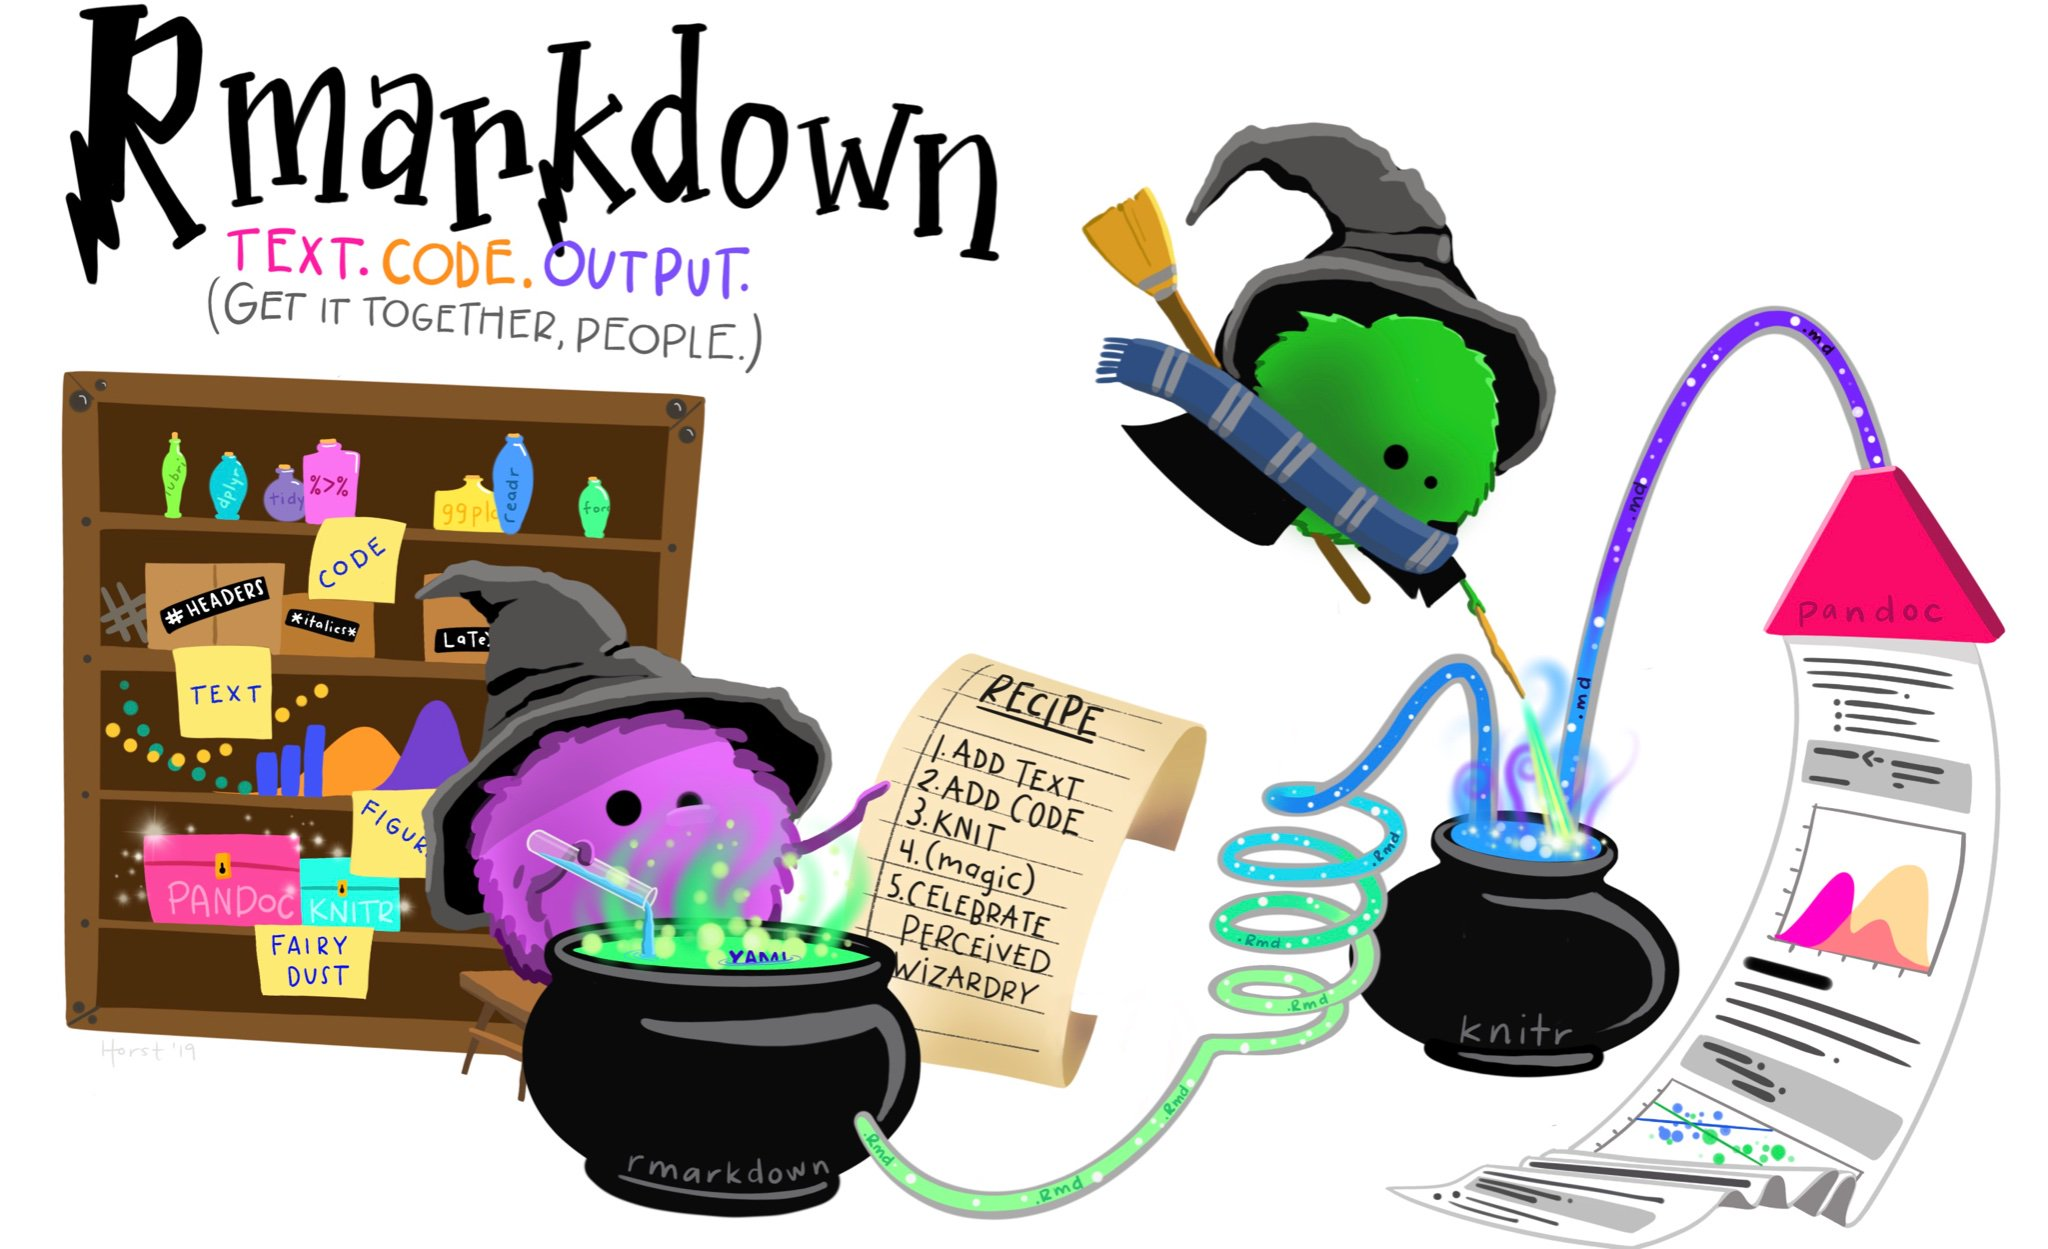
\includegraphics[width=0.8\linewidth]{images/wizard} \caption{courtesy of Allison Horst}\label{fig:unnamed-chunk-2}
\end{figure}

\hypertarget{introduction-to-r}{%
\section{Introduction to R}\label{introduction-to-r}}

\href{https://www.r-project.org/}{R} is the name of the programming language itself and \href{img/rstudio-ide.pdf}{RStudio} is a convenient interface.{]}, which we will be using throughout the course in order to learn how to organise data, produce accurate data analyses \& data visualisations.

Eventually we will also add extra tools like \href{https://www.youtube.com/watch?v=w3jLJU7DT5E}{GitHub} and \href{https://rmarkdown.rstudio.com/}{RMarkdown} for data reproducibility and collaborative programming, check out this short (and very cheesy) intro video.{]}, which are collaboration and version control systems that we will be using throughout the course. More on this in future weeks.

By the end of this module I hope you will have the tools to confidently analyze real data, make informative and beautiful data visuals, and be able to analyse lots of different types of data.

The taught content this autumn will be given to you in several \textbf{worksheets}, these will be added to this dynamic webpage each week.

\hypertarget{getting-around-on-rstudio}{%
\section{Getting around on RStudio}\label{getting-around-on-rstudio}}

\hypertarget{an-intro-to-rstudio}{%
\subsection{An intro to RStudio}\label{an-intro-to-rstudio}}

RStudio

\begin{quote}
Note - people often mix up R and RStudio. R is the programming language (the engine), RStudio is a handy interface/wrapper that makes things a bit easier to use.
\end{quote}

\hypertarget{using-r-studio-cloud}{%
\subsection{Using R Studio Cloud}\label{using-r-studio-cloud}}

RStudio Cloud works in exactly the same way as RStudio, but means you don't have to download any software. You can access the hosted cloud server and your projects through any browser connection (Chrome works best), from any computer.

\hypertarget{get-help}{%
\section{Get Help!}\label{get-help}}

There are a \textbf{lot} of sources of information about using R out there.
Here are a few helpful places to get help when you have an issue, or just to learn more

\begin{itemize}
\item
  The R help system itself - we cover this in @ref(Getting to know R - Week One)
\item
  Vignettes - type \texttt{browseVignettes()} into the console and hit Enter, a list of available vignettes for all the packages we have will be displayed
\item
  \href{https://www.rstudio.com/resources/cheatsheets/}{Cheat Sheets} - available at RStudio.com. Most common packages have an associate cheat sheet covering the basics of how to use them. Download/bookmark ones we will use commonly such as \texttt{ggplot2}, \texttt{Data\ transformation\ with\ dplyr}, \texttt{Data\ tidying\ with\ tidyr} \& \texttt{Data\ import}.
\item
  Google - I use Google constantly, because I continually forget how to do even basic tasks. If I want to remind myself how to round a number, I might type something like \texttt{R\ round\ number} - if I am using a particular package I should include that in the search term as well
\item
  Ask for help - If you are stuck, getting an error message, can't think what to do next, then ask someone. It could be me, it could be a classmate. When you do this it is very important that you \textbf{show the code}, include the \textbf{error message}. ``This doesn't work'' is not helpful. ``Here is my code, this is the data I am using, I want it to do X, and here's the problem I get''.
\end{itemize}

\begin{quote}
Note - It may be daunting to send your code to someone for help. It is natural and common to feel apprehensive, or to think that your code is really bad. I still feel the same! But we learn when we share our mistakes, and eventually you will find it funny when you look back on your early mistakes, or laugh about the mistakes you still occasionally make!
\end{quote}

\hypertarget{getting-to-know-r---week-one}{%
\chapter{Getting to know R - Week One}\label{getting-to-know-r---week-one}}

Go to RStudio Cloud and enter the Project labelled \texttt{Week\ One} - this will clone the project and provide you with your own workspace.

Follow the instructions below to get used to the R command line, and how R works as a language.

\hypertarget{your-first-r-command}{%
\section{Your first R command}\label{your-first-r-command}}

In the RStudio pane, navigate to the console (bottom left) and \texttt{type\ or\ copy} the below it should appear at the \textgreater{}

Hit Enter on your keyboard.

\begin{Shaded}
\begin{Highlighting}[]
\DecValTok{10} \SpecialCharTok{+} \DecValTok{20}
\end{Highlighting}
\end{Shaded}

You should now be looking at the below:

\begin{verbatim}
> 10 + 20
[1] 30
\end{verbatim}

The first line shows the request you made to R, the next line is R's response

You didn't type the \texttt{\textgreater{}} symbol: that's just the R command prompt and isn't part of the actual command.

It's important to understand how the output is formatted. Obviously, the correct answer to the sum \texttt{10\ +\ 20} is \texttt{30}, and not surprisingly R has printed that out as part of its response. But it's also printed out this \texttt{{[}1{]}} part, which probably doesn't make a lot of sense to you right now. You're going to see that a lot. You can think of \texttt{{[}1{]}\ 30} as if R were saying ``the answer to the 1st question you asked is 30''.

\hypertarget{typos}{%
\subsection{Typos}\label{typos}}

Before we go on to talk about other types of calculations that we can do with R, there's a few other things I want to point out. The first thing is that, while R is good software, it's still software. It's pretty stupid, and because it's stupid it can't handle typos. It takes it on faith that you meant to type \emph{exactly} what you did type. For example, suppose that you forgot to hit the shift key when trying to type \texttt{+}, and as a result your command ended up being \texttt{10\ =\ 20} rather than \texttt{10\ +\ 20}. Try it for yourself and replicate this error message:

\begin{Shaded}
\begin{Highlighting}[]
\DecValTok{10} \OtherTok{=} \DecValTok{20}
\end{Highlighting}
\end{Shaded}

\begin{verbatim}
## Error in 10 = 20: invalid (do_set) left-hand side to assignment
\end{verbatim}

What's happened here is that R has attempted to interpret \texttt{10\ =\ 20} as a command, and spits out an error message because the command doesn't make any sense to it. When a \emph{human} looks at this, and then looks down at his or her keyboard and sees that \texttt{+} and \texttt{=} are on the same key, it's pretty obvious that the command was a typo. But R doesn't know this, so it gets upset. And, if you look at it from its perspective, this makes sense. All that R ``knows'' is that \texttt{10} is a legitimate number, \texttt{20} is a legitimate number, and \texttt{=} is a legitimate part of the language too. In other words, from its perspective this really does look like the user meant to type \texttt{10\ =\ 20}, since all the individual parts of that statement are legitimate and it's too stupid to realise that this is probably a typo. Therefore, R takes it on faith that this is exactly what you meant\ldots{} it only ``discovers'' that the command is nonsense when it tries to follow your instructions, typo and all. And then it whinges, and spits out an error.

Even more subtle is the fact that some typos won't produce errors at all, because they happen to correspond to ``well-formed'' R commands. For instance, suppose that not only did I forget to hit the shift key when trying to type \texttt{10\ +\ 20}, I also managed to press the key next to one I meant do. The resulting typo would produce the command \texttt{10\ -\ 20}. Clearly, R has no way of knowing that you meant to \emph{add} 20 to 10, not \emph{subtract} 20 from 10, so what happens this time is this:

\begin{Shaded}
\begin{Highlighting}[]
\DecValTok{10} \SpecialCharTok{{-}} \DecValTok{20}
\end{Highlighting}
\end{Shaded}

\begin{verbatim}
## [1] -10
\end{verbatim}

In this case, R produces the right answer, but to the the wrong question.

\hypertarget{more-simple-arithmetic}{%
\subsection{More simple arithmetic}\label{more-simple-arithmetic}}

One of the best ways to get to know R is to play with it, it's pretty difficult to break it so don't worry too much. Type whatever you want into to the console and see what happens.

If the last line of your console looks like this

\begin{verbatim}
> 10+
+ 
\end{verbatim}

and there's a blinking cursor next to the plus sign. This means is that R is still waiting for you to finish. It ``thinks'' you're still typing your command, so it hasn't tried to execute it yet. In other words, this plus sign is actually another command prompt. It's different from the usual one (i.e., the \texttt{\textgreater{}} symbol) to remind you that R is going to ``add'' whatever you type now to what you typed last time. For example, type \texttt{20} and hit enter, then it finishes the command:

\begin{verbatim}
> 10 +
+ 20
[1] 30
\end{verbatim}

\emph{Alternatively} hit escape, and R will forget what you were trying to do and return to a blank line.

\hypertarget{try-some-maths}{%
\subsection{Try some maths}\label{try-some-maths}}

\begin{Shaded}
\begin{Highlighting}[]
\DecValTok{1}\SpecialCharTok{+}\DecValTok{7}
\end{Highlighting}
\end{Shaded}

\begin{Shaded}
\begin{Highlighting}[]
\DecValTok{13{-}10}
\end{Highlighting}
\end{Shaded}

\begin{Shaded}
\begin{Highlighting}[]
\DecValTok{4}\SpecialCharTok{*}\DecValTok{6}
\end{Highlighting}
\end{Shaded}

\begin{Shaded}
\begin{Highlighting}[]
\DecValTok{12}\SpecialCharTok{/}\DecValTok{3}
\end{Highlighting}
\end{Shaded}

Raise a number to the power of another

\begin{Shaded}
\begin{Highlighting}[]
\DecValTok{5}\SpecialCharTok{\^{}}\DecValTok{4}
\end{Highlighting}
\end{Shaded}

As I'm sure everyone will probably remember the moment they read this, the act of multiplying a number \(x\) by itself \(n\) times is called ``raising \(x\) to the \(n\)-th power''. Mathematically, this is written as \(x^n\). Some values of \(n\) have special names: in particular \(x^2\) is called \(x\)-squared, and \(x^3\) is called \(x\)-cubed. So, the 4th power of 5 is calculated like this:
\[
5^4 = 5 \times 5 \times 5 \times 5 
\]

\hypertarget{perform-some-combos}{%
\subsection{Perform some combos}\label{perform-some-combos}}

Perform some mathematical combos, noting that the order in which R performs calculations is the standard one.

That is, first calculate things inside \textbf{B}rackets \texttt{()}, then calculate \textbf{O}rders of (exponents) \texttt{\^{}}, then \textbf{D}ivision \texttt{/} and \textbf{M}ultiplication \texttt{*}, then \textbf{A}ddition \texttt{+} and \textbf{S}ubtraction \texttt{-}.

Notice the different outputs of these two commands.

\begin{Shaded}
\begin{Highlighting}[]
\DecValTok{3}\SpecialCharTok{\^{}}\DecValTok{2{-}5}\SpecialCharTok{/}\DecValTok{2}
\end{Highlighting}
\end{Shaded}

\begin{Shaded}
\begin{Highlighting}[]
\NormalTok{(}\DecValTok{3}\SpecialCharTok{\^{}}\DecValTok{2{-}5}\NormalTok{)}\SpecialCharTok{/}\DecValTok{2}
\end{Highlighting}
\end{Shaded}

Similarly if we want to raise a number to a fraction, we need to surround the fraction with parentheses ()

\begin{Shaded}
\begin{Highlighting}[]
\DecValTok{16}\SpecialCharTok{\^{}}\DecValTok{1}\SpecialCharTok{/}\DecValTok{2}
\end{Highlighting}
\end{Shaded}

\begin{Shaded}
\begin{Highlighting}[]
\DecValTok{16}\SpecialCharTok{\^{}}\NormalTok{(}\DecValTok{1}\SpecialCharTok{/}\DecValTok{2}\NormalTok{)}
\end{Highlighting}
\end{Shaded}

The first one calculates 16 raised to the power of 1, then divided this answer by two. The second one raises 16 to the power of a half. A big difference in the output.

\begin{quote}
**Note - While the cursor is in the console, you can press the up arrow to see all your previous commands.
You can run them again, or edit them. Later on we will look at scripts, as an essential way to re-use, store and edit commands.
\end{quote}

\hypertarget{storing-outputs}{%
\section{Storing outputs}\label{storing-outputs}}

\hypertarget{quitting-r}{%
\subsection{Quitting R}\label{quitting-r}}

There's one last thing I should cover in this chapter: how to quit R. When I say this, I'm not trying to imply that R is some kind of pathological addition and that you need to call the R QuitLine or wear patches to control the cravings (although you certainly might argue that there's something seriously pathological about being addicted to R). I just mean how to exit the program. Assuming you're running R in the usual way (i.e., through RStudio or the CLoud), then you can just shut down the application in the normal way by clicking the close windown button. However, R also has a function, called \texttt{q()} that you can use to quit, which is pretty handy if you're running R in a terminal window e.g.~when using servers - we will cover some of this later in the course.

Regardless of what method you use to quit R, when you do so for the first time R will probably ask you if you want to save the ``workspace image''. I talked about this in one of my videos, it's annoying and occasionally introduces complications, so if prompted it is usually better to click \texttt{NO} (but don't worry if you hit the wrong button).

What does this actually \emph{mean}? What's going on is that R wants to know if you want to save \textbf{all} those variables that you've been creating, so that you can use them later. This sounds like a great idea, so it's really tempting to type \texttt{y} or click the ``Save'' button. To be honest though, I very rarely do this, and it kind of annoys me a little bit\ldots{} what R is \emph{really} asking is if you want it to store these variables in a ``default'' data file (R.data), which it will automatically reload for you next time you open R. But as we will learn to work with scripts, this is unnecessary.

In fact, every time I install R on a new machine one of the first things I do is change the settings so that it never asks me again. You can do this in RStudio really easily: use the menu system to find the RStudio option; the dialog box that comes up will give you an option to tell R never to whine about this again.

We practice what we preach! This site is created with Git and R markdown, using the \href{https://github.com/rstudio/bookdown/}{\texttt{bookdown}} package. Go ahead and \href{https://github.com/jennybc/happy-git-with-r}{peek behind the scenes}.

Long-term, you should understand more about what you are doing. Rote clicking in RStudio may be a short-term survival method but won't work for long.

\begin{itemize}
\item
  \href{https://try.github.io/levels/1/challenges/1}{trygit} is to (command line) Git as \href{http://swirlstats.com}{swirl} is to R. Learn by doing, in small bites.
\item
  The book \href{http://git-scm.com/book}{Pro Git} is fantastic and comprehensive.
\item
  \href{https://www.manning.com/books/git-in-practice}{Git in Practice} by Mike McQuaid is an more approachable book, probably better than Pro Git for most people starting out. Ancillary materials \href{https://github.com/MikeMcQuaid/GitInPractice}{on GitHub}.
\item
  \href{https://speakerdeck.com/alicebartlett/git-for-humans}{Git for Humans} is a great set of slides by \href{https://alicebartlett.co.uk}{Alice Bartlett}, originally delivered in 2016 at UX Brighton.
\item
  \href{http://training.github.com/kit/}{GitHub's own training materials} may be helpful. They also point to \href{https://help.github.com/articles/what-are-other-good-resources-for-learning-git-and-github}{many other resources}
\item
  Find a powerful Git client (chapter \ref{git-client}) if you'd like to minimize your usage of Git from the command line.
\item
  Hadley Wickham's book \href{http://r-pkgs.had.co.nz}{R Packages} has an excellent \href{http://r-pkgs.had.co.nz/git.html}{chapter on the use of Git, GitHub, and RStudio} in R package development. He covers more advanced usage, such as commit best practices, issues, branching, and pull requests.
\item
  Ten Simple Rules for Taking Advantage of Git and GitHub \url{http://journals.plos.org/ploscompbiol/article?id=10.1371/journal.pcbi.1004947}
\item
  RStudio's guide \href{https://support.rstudio.com/hc/en-us/articles/200532077-Version-Control-with-Git-and-SVN}{Version Control with Git and SVN}
\item
  The book \emph{\href{http://shop.oreilly.com/product/0636920018025.do}{Team Geek}} has insightful advice for the human and collaborative aspects of version control. It proposes Git strategies suited to different characteristics of teams.
\end{itemize}

  \bibliography{book.bib,packages.bib}

\end{document}
